\section{\blue{Dataset Construction}}
\label{sec:res_dataset}

The dataset construction followed a sequence of incremental steps, following the methodology presented on \refCap{sec:method_dataset}. The proposed labeling method assumes that a model trained with the current iteration of the dataset will be able to create better (i.e. more precise) labels if compared to training with the previous iteration (should have less data), which will then speedup the human annotation process. \refTab{tab:dataset_iterations} shows this behavior. This table details every iteration of the training loop: the achieved number of documents, followed by number of classes, and the similarity between what was automatically clustered versus the resulting human annotated labels. Each iteration begins with a automatic clustering produced by a model trained on the dataset achieved by the previous iteration. The first iteration takes the dataset from a previous work~\cite{10.1007/978-3-032-09368-4_12} and creates a new, independent dataset.

\begin{table}[ht]
\centering
\begin{tabular}{ccccc}
    \toprule
    Iteration & Number of Documents & Number of Classes & \gls{ARI} & \gls{NMI} \\
    \midrule
    1 & 10,659 & 512 & 0.131 & 0.665 \\
    2 & 12,246 & 560 & 0.141 & 0.650 \\
    3 & 17,295 & 665 & 0.440 & 0.784 \\
    \bottomrule
\end{tabular}
\caption{Iterative dataset construction metrics. Each row shows information of a iteration of the dataset, such as the total number of documents and classes in the dataset at that iteration. ARI and NMI are similarity metrics between the automatic labeling process, and the final, human annotated labels.}
\label{tab:dataset_iterations}
\end{table}

The table shows an increase in cluster similarity with the growth of the dataset. In particular, the increase from the second to the third iteration is greater than the increase from the first to the second. It is possible that the data achieved by the first iteration had the same overall quality than the data achieved by the previous work, meaning that models trained in these datasets achieved similar behavior. The labeling loop then follow with a leap of cluster quality in the third iteration, revealing evidence that the labeling method can optimize the manual process. Furthermore, the second and the third iterations both lasted the same duration, and yet, the second iteration achieved 1,587 new documents, and the third, 5,049. This is an empirical evidence that the cluster similarity is inversely related to the time spent per document on the manual annotation process. The remaining experiments on this work are done with the last iteration of the dataset.

\section{Hyperparameter search}
\label{sec:results}

Before making a proper benchmark, a hyperparameter search is necessary. Most hyperparameters are already set, as they are taken from the original works (see \refCap{sec:experimental_setup}), but hyperparameters related to the metric-learning nature have not been set. \refTab{tab:tuning_raw} shows the search for the remaining configurations: the architecture edition, the distance metric and the embedding size.

\begin{table}[ht]
\centering
\setlength{\tabcolsep}{4pt}
\footnotesize
\begin{tabular}{llcccccc|ccccccc}
\toprule
& & \multicolumn{6}{c}{Euclidean} & \multicolumn{6}{c}{Cosine} \\
\cmidrule(lr){3-8} \cmidrule(lr){9-14}
Model & Ed. & 16 & 32 & 64 & 128 & 256 & 512 & 16 & 32 & 64 & 128 & 256 & 512 \\
\midrule
AlexNet                 &   & 24.71 & 20.45 & 34.81 & 33.61 & 31.07 & 22.31 & 21.21 & 20.21 & 21.62 & 18.44 & 22.14 & \underline{\textbf{15.26}} \\
\midrule
\multirow{4}{*}{VGG}    & 11    & 19.35 & 32.73 & 9.03 & 31.68 & 30.82 & 34.59 & 22.80 & 29.38 & 20.23 & 22.02 & 29.31 & 26.39 \\
                        & 13    & 22.38 & 8.83 & 24.05 & 14.82 & 33.05 & 11.69 & 18.22 & 23.61 & 13.85 & 19.59 & 24.22 & 30.01 \\
                        & 16    & 7.63 & 4.82 & 30.80 & 12.57 & 23.39 & 8.90 & 12.01 & 27.76 & 22.65 & 30.23 & 25.68 & 32.63 \\
                        & 19    & 13.26 & 1.81 & 29.79 & 18.08 & 27.67 & 11.86 & 23.48 & 23.17 & 19.69 & 21.18 & 1.66 & \underline{\textbf{1.57}} \\
\midrule
\multirow{5}{*}{ResNet} & 18    & 3.52 & 7.07 & 9.00 & 7.05 & 3.40 & 1.66 & 19.35 & 11.69 & 2.94 & 2.35 & 1.64 & 2.64 \\
                        & 34    & 9.10 & 10.30 & 7.36 & 8.07 & 17.71 & 3.30 & 3.23 & 4.82 & 1.54 & 5.48 & \underline{\textbf{0.49}} & 0.61 \\
                        & 50    & 7.07 & 26.47 & 11.69 & 4.01 & 23.24 & 14.75 & 15.95 & 17.25 & 4.31 & 6.04 & 10.37 & 10.10 \\
                        & 101   & 21.80 & 19.06 & 20.72 & 21.23 & 31.99 & 19.06 & 13.04 & 6.73 & 3.84 & 2.42 & 7.75 & 24.93 \\
                        & 152   & 7.14 & 4.77 & 14.24 & 13.72 & 5.70 & 16.85 & 4.26 & 8.98 & 2.62 & 15.63 & 13.70 & 9.34 \\
\midrule
\multirow{2}{*}{MobileNet} & S. & 7.44 & 13.60 & 48.29 & 16.24 & 29.87 & 39.97 & 20.38 & 6.36 & 5.53 & 14.04 & 5.14 & 5.60 \\
                           & L. & 22.82 & 43.79 & 38.01 & 46.16 & 44.32 & 31.60 & 17.34 & 16.44 & 17.10 & 10.57 & \underline{\textbf{5.09}} & 12.84 \\
\midrule
\multirow{4}{*}{EfficientNet} & 0  & 7.61 & 1.00 & 5.68 & 1.88 & 14.46 & \underline{\textbf{0.73}} & 2.67 & 5.53 & 3.96 & 8.73 & 2.62 & 2.81 \\
                              & 1  & 4.99 & 7.44 & 5.31 & 3.33 & 6.73 & 5.09 & 2.54 & 4.84 & 3.86 & 5.75 & 1.37 & 2.40 \\
                              & 2  & 3.42 & 4.11 & 4.26 & 3.99 & 2.15 & 13.50 & 4.87 & 3.11 & 2.59 & 12.77 & 4.26 & 6.65 \\
                              & 3  & 19.50 & 5.28 & 4.26 & 8.71 & 11.15 & 8.00 & 10.10 & 4.35 & 3.99 & 12.87 & 10.59 & 6.09 \\
\midrule
\multirow{2}{*}{ViT}    & B.  & 29.43 & 33.19 & 17.95 & 28.01 & 25.15 & 24.66 & 30.26 & 37.77 & 38.60 & 26.83 & 18.62 & 32.27 \\
                        & L. & 19.32 & 27.81 & 28.69 & \underline{\textbf{16.81}} & 22.60 & 21.72 & 25.76 & 18.15 & 40.17 & 38.43 & 22.38 & 30.53 \\
\bottomrule
\end{tabular}
\caption{Results of the hyperparameter search for each arquitecture in \gls{EER}. Searching for: the architecture edition (e.g. ResNet-18 or ResNet-34), the distance metric (Euclidean or cosine), and the output embedding size.}
\label{tab:tuning_raw}
\end{table}

The experiments in \refTab{tab:tuning_raw} use the first fold of the cross-validation as the train and validation splits, and the resported values are from the independent test split. This table is used to find the best possible parameter configuration for each architecture, and the remaining experiments on this work are done with the best hyperparameters found. To better analyse these results, this table is split into other three different tables.

\begin{table}[ht]
\centering
\setlength{\tabcolsep}{4pt}
\begin{tabular}{ccc|cc|cc}
& \multicolumn{2}{c}{Euclidean} & \multicolumn{2}{c}{Cosine} & \multicolumn{2}{c}{Both} \\
\cmidrule(lr){2-3} \cmidrule(lr){4-5} \cmidrule(lr){6-7}
Embedding Size & Mean & Std & Mean & Std & Mean & Std \\
\midrule
16  & 13.92 & 8.39 & 14.86 & 8.69 & 14.39 & 8.43 \\
32  & 15.14 & 12.81 & 15.01 & 10.33 & 15.07 & 11.47 \\
64  & 19.39 & 13.77 & 12.81 & 11.99 & 15.92 & 13.10 \\
128 & 16.11 & 12.14 & 15.19 & 9.96 & 15.65 & 10.95 \\
256 & 21.36 & 11.91 & \underline{\textbf{11.50}} & 9.74 & 16.43 & 11.83 \\
512 & 16.13 & 11.37 & 14.04 & 11.96 & 15.08 & 11.55 \\
\midrule
All & 16.99 & 11.83 & 13.89 & 10.37 & 15.42 & 11.20 \\
\bottomrule
\end{tabular}
\caption{Average performance in \gls{EER} over each possible output dimension, considering the Euclidean distance, the Cosine distance, and considering both distances. The last row considers every embedding size, to measure the best average distance metric.}
\label{tab:outdim_agg}
\end{table}

% revise esse aqui
\refTab{tab:outdim_agg} shows the average \gls{EER} for each combination of metric distance and embedding size. We can see that the best overall combination is a embedding of size 256, and using the cosine distance. We can see in the last row, where the results are averaged across every embedding size, that the cosine distance is indeed the best overall metric distance, with a absolute difference of 3.10\% \gls{EER} from the euclidian distance. This is evidence that most architectures used in these experiments work better with the cosine distance for this problem. The last two columns on this table brings the average \gls{EER} for each embedding size, averaging the distance metrics. In these columns, we can see that the smaller embedding size used, 16, is actually the best overall, with the lowest standard deviation. A smaller embedding size implies in a smaller feature space, therefore, it is possible that models trained with 16 embedding size are less prone to overfitting, achieving stable but moderate results. Higher embedding sizes, while more prone to overfitting, also hold the potential handle more classes without entanglement. We can see this behavior in \refTab{tab:tuning_raw}: while embedding size of 16 is the best average value, it was not once the best hyperparameter for any architecture, and most best configurations use 256 or 512 embedding size.

\begin{table}[ht]
    \centering
    \setlength{\tabcolsep}{4pt}
    \begin{tabular}{ccc|cc|cc}
        & \multicolumn{2}{c}{Euclidean} & \multicolumn{2}{c}{Cosine} & \multicolumn{2}{c}{Both} \\
        \cmidrule(lr){2-3} \cmidrule(lr){4-5} \cmidrule(lr){6-7}
        Architecture & Mean & Std & Mean & Std & Mean & Std \\
        \midrule
        AlexNet         & 27.83 & 6.12 & 19.81 & 2.58 & 23.82 & 6.13 \\
        VGG             & 19.32 & 10.30 & 21.72 & 7.96 & 20.52 & 9.19 \\
        ResNet          & 12.30 & 8.01 & 8.01 & 6.26 & 10.08 & 7.42 \\
        MobileNetV3     & 31.84 & 13.93 & 11.37 & 5.69 & 21.61 & 14.75 \\
        EfficientNet    & 6.36 & 4.50 & 5.39 & 3.30 & 5.87 & 3.93 \\
        ViT             & 24.61 & 5.06 & 29.98 & 7.81 & 27.30 & 6.99 \\
        \bottomrule
    \end{tabular}
    \caption{Average performance in \gls{EER} over each possible architecture, considering the Euclidean distance, the Cosine distance, and considering both distances.}
    \label{tab:architecture_agg}
\end{table}

\refTab{tab:architecture_agg} shows the average \gls{EER} for each combination of distance function and chosen architecture. We can see that the best combination of architecture and metric distance is EfficientNet with cosine distance. Most architectures perform better with cosine distance, with the exception of \gls{ViT} and VGG. MobileNet performed particularly bad with the euclidian distance, with almost three times the \gls{EER} if compared against using the cosine distance. \refTab{tab:tuning_raw} shows that some experiments with this combination got near 50\% \gls{EER}, a score that would be as bad as a completely random decision. In these cases, the trained models mostly did not learn across all the 300 epochs they were trained on. Again, the last two columns shows the performance of each architecture, independently of the chosen distance metric. The best overall architecture in these experiments are the EfficientNet variants, followed by ResNet and VGG.

\begin{table}[ht]
\centering
\setlength{\tabcolsep}{4pt}
\footnotesize 
\begin{tabular}{ccc|cc|cc|cc|cc|cc}
& \multicolumn{2}{c}{16} & \multicolumn{2}{c}{32} & \multicolumn{2}{c}{64} & \multicolumn{2}{c}{128} & \multicolumn{2}{c}{256} & \multicolumn{2}{c}{512} \\
\cmidrule(lr){2-3} \cmidrule(lr){4-5} \cmidrule(lr){6-7} \cmidrule(lr){8-9} \cmidrule(lr){10-11} \cmidrule(lr){12-13}
Architecture & Mean & Std & Mean & Std & Mean & Std  & Mean & Std & Mean & Std & Mean & Std\\
\midrule
AlexNet         & 22.96 & 2.47 & 20.33 & 0.17  & 28.22 & 9.32  & 26.03 & 10.72 & 26.60 & 6.31  & 18.79 & 4.98 \\
VGG             & 17.39 & 5.82 & 19.01 & 12.02 & 21.26 & 7.38  & 21.27 & 6.76  & 24.47 & 9.79  & 19.71 & 12.60 \\
ResNet          & 10.45 & 6.73 & 11.71 & 7.10  & 7.83  & 6.17  & 8.60  & 6.26  & 11.60 & 10.19 & 10.33 & 8.37 \\
MobileNetV3     & 16.99 & 6.75 & 20.05 & 16.39 & 27.23 & 19.44 & 21.75 & 16.44 & 21.10 & 19.39 & 22.50 & 15.99 \\
EfficientNet    & 6.96  & 5.68 & 4.46  & 1.88  & 4.24  & 0.94  & 7.25  & 4.20  & 6.67  & 4.88  & 5.66  & 3.99 \\
ViT             & 26.19 & 4.98 & 29.23 & 8.43  & 31.35 & 10.28 & 27.52 & 8.84  & 22.19 & 2.69  & 27.29 & 4.94 \\
\bottomrule
\end{tabular}
\caption{Average performance in \gls{EER} over each possible architecture, considering each output dimension.}
\label{tab:architecture_dim_agg}
\end{table}

Finally, the \ref{tab:architecture_dim_agg} shows the performance of each architecture, for each possible embedding size. This table shows some of the behaviors pointed out in the two previous paragraphs: embedding size of value 16 having lower overall standard deviation and EfficientNet achieving the lowest average \gls{EER}. The best combination of embedding size and architecture, in average, is EfficientNet with size 64, and is different from the best hyperparameter combination found on \refTab{tab:tuning_raw}, which is using embedding size 512. This shows, again, that while bigger embeddings may increase the potential for better models, it can also increase the variability of the results. \refFig{fig:boxplot} shows a boxplot of the \gls{EER} in relation to the embedding size, across all experiments shown in \refTab{tab:tuning_raw}. Note that the error oscilates across the size options and is neither strictly increasing or decreasing, and the most stable parameter is still the 16 embedding size.

\begin{figure}
    \centering
    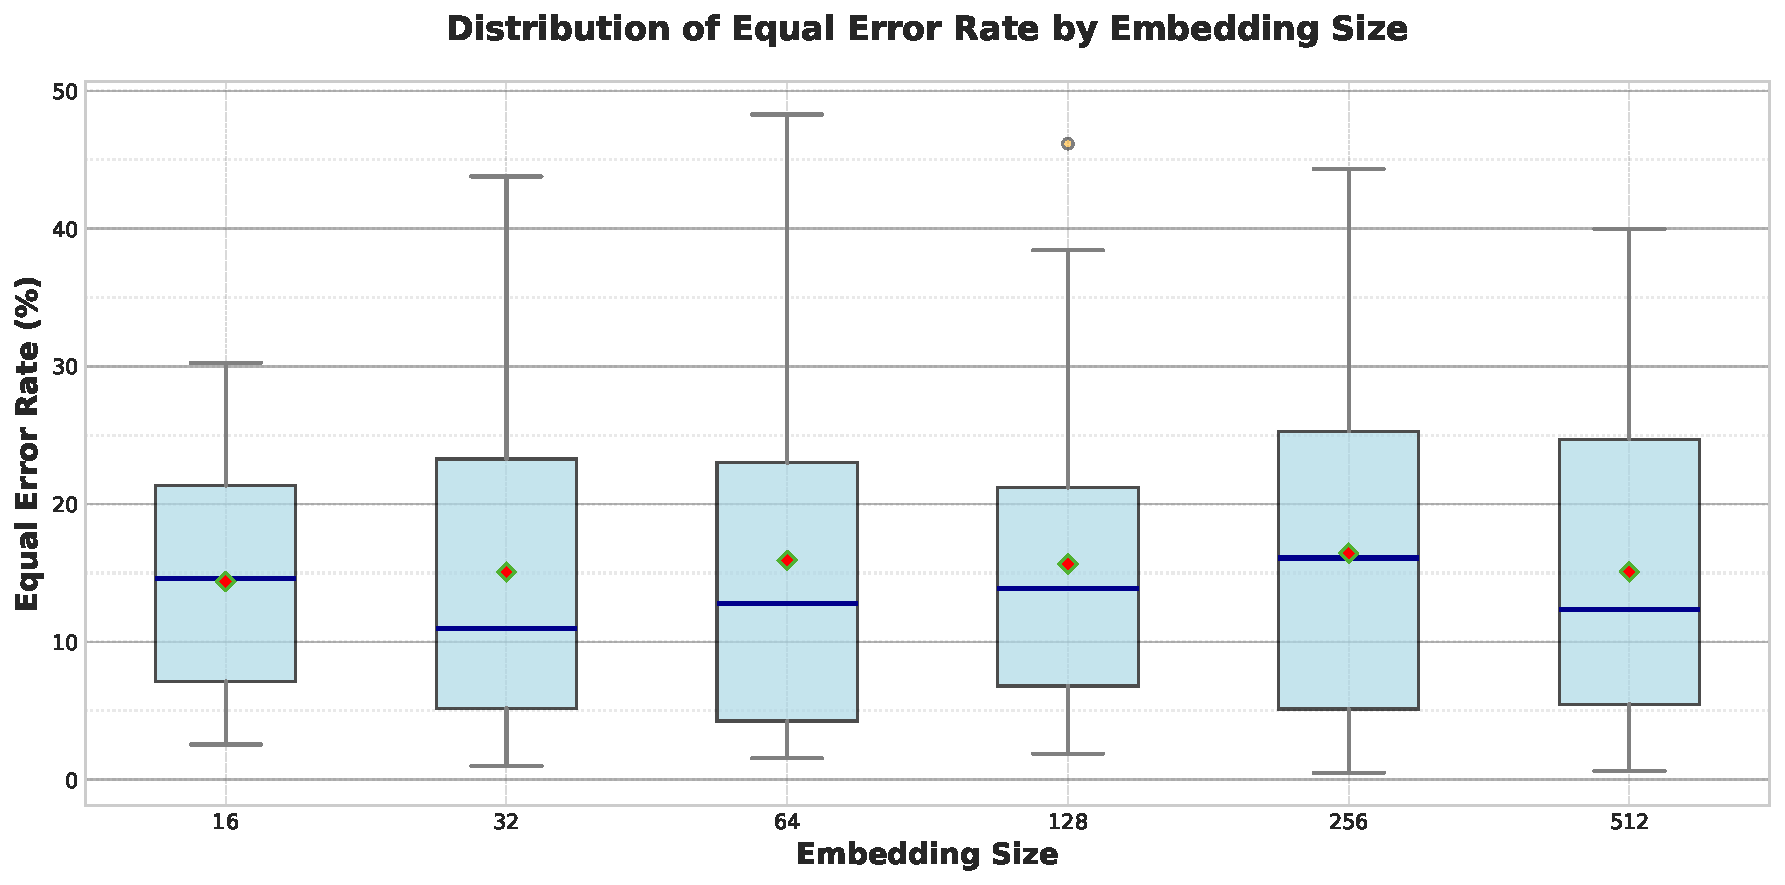
\includegraphics[width=\textwidth]{images/boxplot_eer_embedding_size.pdf}
    \caption{Boxplot of the \gls{EER} over the different chosen embedding sizes. In each box, the blue line represents the median value, and the red shape represents the average value.}
    \label{fig:boxplot}
\end{figure}

\section{Benchmark}

This sections's discussion revolves around Table \ref{tab:res}, where the results of every trained model are presented. The table shows the average EER value of the cross-validation in both scenarios, as well as the average performance of each fold on the independent test set. \red{OQ MAIS?}

\begin{table}[ht]
    \centering
    \setlength{\tabcolsep}{6pt}
    \begin{tabular}{lclcccc}
        \toprule
        & & & \multicolumn{2}{c}{\gls{ZSL}} & \multicolumn{2}{c}{Test \gls{ZSL}} \\
        \cmidrule(lr){4-5} \cmidrule(lr){6-7}
        Architecture           & Edition & Params & Mean   & Std   & Mean   & Std   \\
        \midrule
        AlexNet                & -       &  -     & -     & -    & -     & -    \\
        VGG                    & -       &  -     & -     & -    & -     & -    \\
        ResNet                 & -       &  -     & -     & -    & -     & -    \\
        MobileNetV3            & -       &  -     & -     & -    & -     & -    \\
        EfficientNet           & -       &  -     & -     & -    & -     & -    \\
        \gls{ViT}              & -       &  -     & -     & -    & -     & -    \\
        \bottomrule
    \end{tabular}
    \caption{Comparative performance between different visual backbones. Following the columns: the architecture name, the architecture edition, cross-validation over the \gls{ZSL} scenario, cross-validation over the \gls{GZSL} scenario, test performance on the \gls{ZSL} scenario, and test performance over the \gls{GZSL} scenario. Every value is a mean EER (\%) value over the five \gls{CV} folds.}
    \label{tab:res}
\end{table}

\subsection{Visual Models}
\label{sec:visual_models}

\red{Among visual models, smaller and more cost-efficient architectures outperformed larger ones. This trend is evident in different ResNet variants: ResNet-18 and ResNet-34 showed strong performance, while larger versions (ResNet-50, ResNet-101, and ResNet-152) performed progressively worse. Additionally, the \gls{ViT}, despite excelling on datasets like ImageNet \cite{deng_imagenet_2009}, was the worst-performing model in this task, both architectures (\gls{ViT}-b and \gls{ViT}-l) achieving over three times the amount of error, in comparison with EfficientNet-b1 in the ZSL scenario. These larger models overfitted to the training data, with some reaching 0\% train error in certain epochs while maintaining a high validation error. The most likely cause of this behavior is the dataset size—LA-CDIP contains only 4,993 documents, with approximately two-thirds used for training in each fold. However, techniques such as tuple mining and data augmentation could help mitigate this effect by increasing the diversity of training samples and improving feature learning. The overall best performing models on this benchmark are the ResNet-18, achieving a $1.54\%$ error rate on the GZSL scenario, and EfficientNet-b0, achieving a $3.93\%$ error rate on the ZSL scenario. Both models offer a balance in size, achieving a good generalization of the problem while also learning the intricacies the task demands.}

\begin{figure}[htbp]
    \centering
    \begin{minipage}{0.4\linewidth}
        \centering
        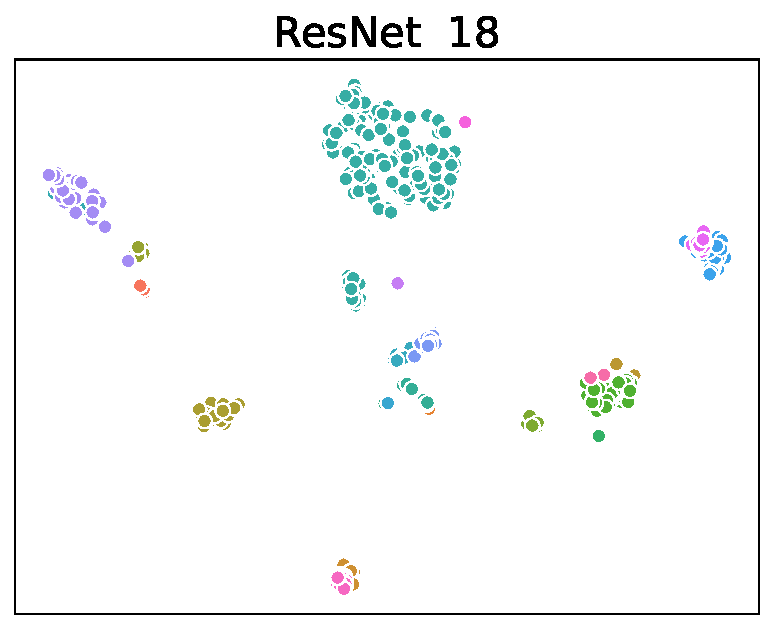
\includegraphics[width=\linewidth]{images/ResNet.csv_18_0.pdf}
        % \caption{Similar Comparison}
    \end{minipage}
    \begin{minipage}{0.4\linewidth}
        \centering
        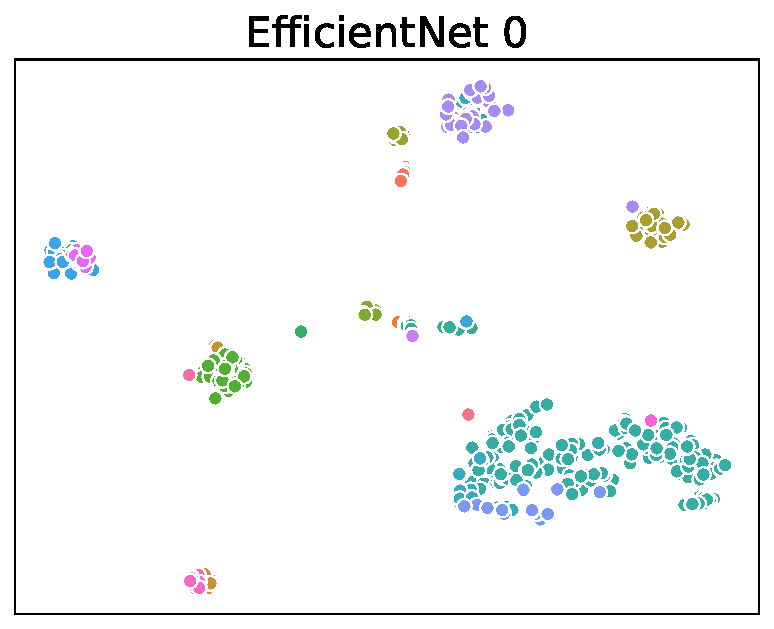
\includegraphics[width=\linewidth]{images/EfficientNet.csv_0_0.pdf}
        % \caption{Different Comparison}
    \end{minipage}
    \begin{minipage}{0.4\linewidth}
        \centering
        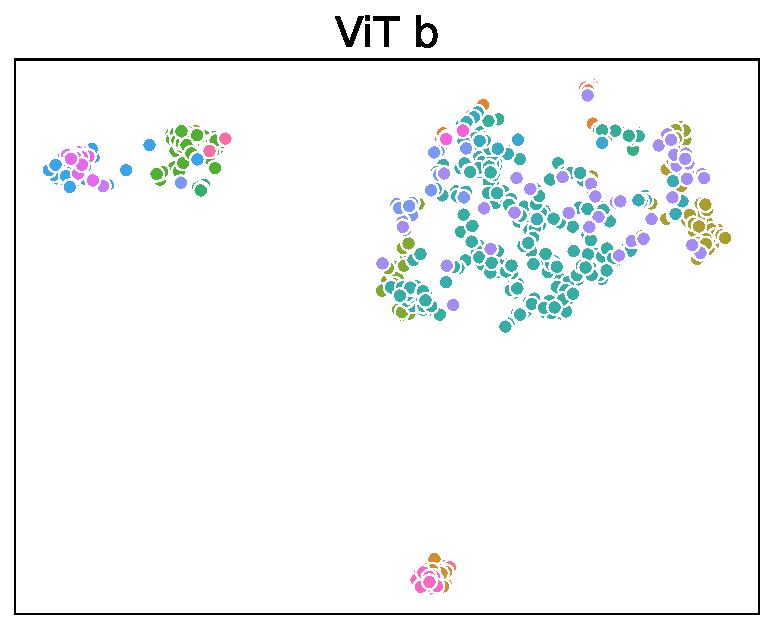
\includegraphics[width=\linewidth]{images/ViT.csv_b_0.pdf}
        % \caption{Different Comparison}
    \end{minipage}
    \begin{minipage}{0.4\linewidth}
        \centering
        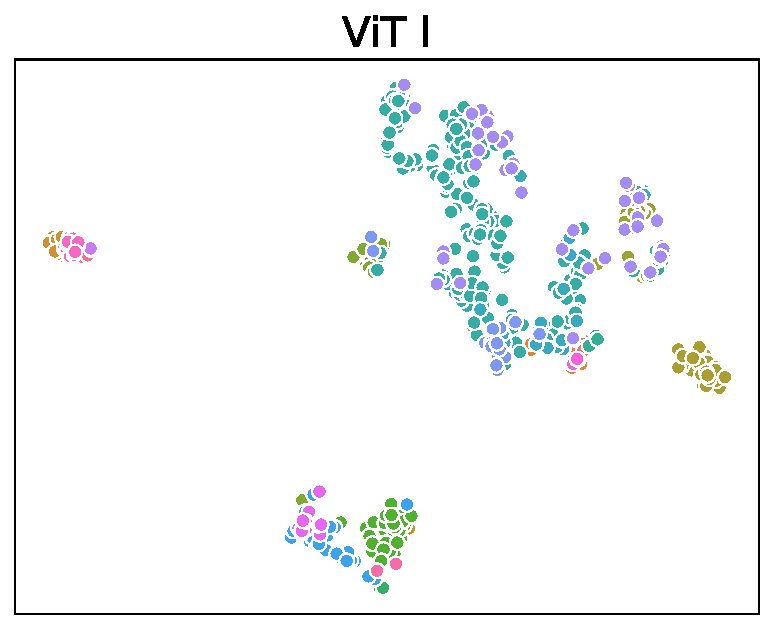
\includegraphics[width=\linewidth]{images/ViT.csv_l_0.pdf}
        % \caption{Different Comparison}
    \end{minipage}
    \caption{TSNE visualization of the Test ZSL scenario. These models were trained on the same cross-validation fold. Each dot represents a document positioned in this two-dimensional space through TSNE dimensionality reduction. Each color represents a different class.\label{fig:tsne}}
\end{figure}

\red{Comparing the \gls{ZSL} and the \gls{GZSL} results, the \gls{GZSL} consistently gives better results. This is expected, since half of the validation set on each fold is composed of classes seen in training. The biggest discrepancies between the two modalities can be seen in the largest models, where the overfitting damage is mitigated by the easier scenario. Even so, the best performance on the \gls{GZSL} scenario is usually connected with a good performance on the \gls{ZSL} scenario.}

\red{In the test scenarios, the reported values represent the mean performance across all folds, evaluated on the same set. Since this is a Zero-shot data split, there is inherently a high variance over the different splits, since they test on entirely different patterns each fold. By chance, the \gls{ZSL} test split is more challenging than average, resulting in higher error rates for most models relative to the mean cross-validation error rate. The test \gls{GZSL} scenario follows the opposite reasoning.}


\section{Industry Uses}

% TODO: Esta seção sobre "Industry Uses" parece mais apropriada para um capítulo
% de Discussão ou Conclusão, pois não apresenta resultados experimentais, mas sim
% possíveis aplicações práticas. Considere mover para o capítulo de Conclusão
% ou criar uma seção de "Discussão" separada.

With the trained models shown in this chapter, an industry system can leverage the metric learning nature of the solution to achieve zero-shot \gls{DIC} in a couple of different ways. First, this model can be used in a verification system, within the same framework used for testing: given a document reference, and with a predefined acceptance threshold, a query document must be accepted if the distance to the reference is smaller than the threshold, and rejected otherwise. As mentioned in \ref{1-Introdução}, this task can be viewed as a binary classification problem, as the system will either accept or reject the document.

Second, the model can be used in an identification system, which becomes similar to a multiclass classification problem: given a document reference for each available class, and with a predefined acceptance threshold, a query document must be assigned to the closest class with respect to the embedding distances, or detected as outside of the label space if no class is within the predefined threshold. \refFig{fig:ver_ind} illustrates the difference between the verification and identification tasks.

\begin{figure*}[ht!]
    \begin{subfigure}[b]{0.35\textwidth}
        \centering
        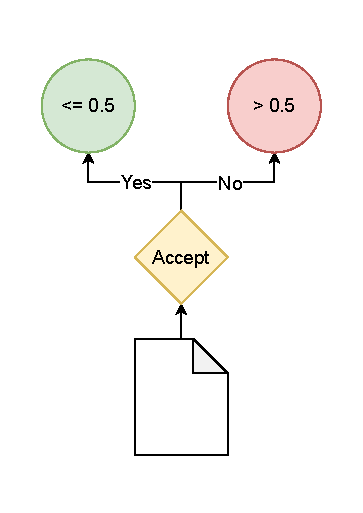
\includegraphics[width=\textwidth]{images/verification.drawio.pdf}
        \caption{Verification task.}
        \label{fig:verification_example}
    \end{subfigure}
    \hfill
    \begin{subfigure}[b]{0.62\textwidth}
        \centering
        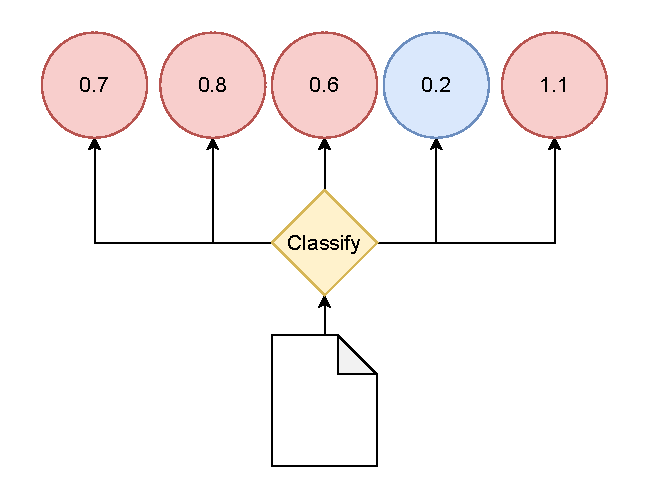
\includegraphics[width=\textwidth]{images/identification.drawio.pdf}
        \caption{Identification task.}
        \label{fig:identification_example}
    \end{subfigure}
    \caption{Comparative illustration between the verification (a) and identification (b) tasks. The verification system approves documents when the distance between the references and the query that is lower than or equal $0.5$, and rejects otherwise. The identification system chose the nearest neighbor to classify the query document.}
    \label{fig:ver_ind}
\end{figure*}

Both tasks can be facilitated by a few design choices. For example, using multiple ground-truth references per class and computing the distance between the query document and the class centroid can improve classification robustness, as it prevents outlier samples from disproportionately representing an entire class. This decision demands more human annotation per class.

Another possible choice is to use a different threshold for each class. While the model is trained to have all classes share the same acceptance threshold, it is natural that some classes in a real-world scenario have less intra-class variance than others. This, of course, increases the maintenance required per class registered in the system, as calculating a unique threshold demands testing. On the other hand, it may be of interest to change the threshold in order to increase the false rejection rate in scenarios where rejecting a correct document is cheaper than accepting an incorrect document, for example.

All these examples share the same need for a database to store the references. It is possible to store the embeddings directly, instead of the document itself, to reduce the number of inferences the model must process. In the verification scenario, the complexity of an inference should increase linearly with the number of references in the class, i.e., the time to calculate the centroid of the class, $O(r)$, where $r$ is the number of references in a given class (the centroid coordinates can be stored to save time). Following the same strategy, in the identification scenario, along with the cost to calculate the centroid, there is also the cost of comparisons per class to find the nearest neighbor, which results in $O(rc)$, where $c$ is the number of classes in the system.
